\chapter{Implementierung}

\section{Hardware}

Für die Testanwendungen wurde ein Knoten definiert, welcher am DicePhyMacHost aus dem Modul Applicationclustering orientiert ist. Dieser wiederum erbt vom Mixim-Knoten WirelessNodeBatteryNetwl. Er beinhaltet sowohl den Funktransreceiver\\
 Nic802154\_TI\_CC2420A, als auch eine Batteriemodul. \\
 Der Sensor\_Wakeup\_DicePhyMacHost enthält zusätzlich dazu die Sensorik aus dem Modul SensorTechnology, welchem im nächsten Abschnitt erläutert wird. Außerdem wurde der Nic802154\_TI\_CC2420A durch den Receiver \\
 Wakeup\_Nic802154\_TI\_CC2420A ersetzt, welcher neben der Standardfunktionalität des Funktransceiver auch noch einen Wakeupreceiver implementiert. Dafür wurde das Modul WakeUpRecv verwendet.

\begin{figure}[htbp]
\centering
\caption{Aufbau Netzwerkknoten}
\label{fig:routingbsp}
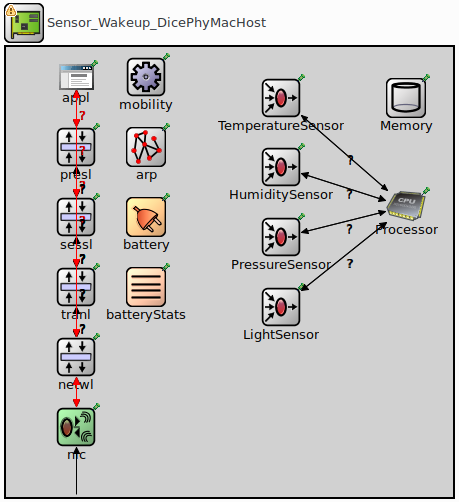
\includegraphics[width=0.3\textwidth]{knoten}
\end{figure}

\subsection{Sensorik}

Das Modul SensorTechnology wurde in der Bachelorarbeit \textit{Modellierung und Integration von Sensorknoten in einer Simulationsumgebung} implementiert. Es stellt die Hardware für die Simulation von der Sensorik bereit, das beinhaltet einen Speicher, einen Prozessor und vier unterschiedliche Sensoren. Der Energieverbrauch der Hardware kann modular definiert werden, es benötigt daher auch eine Energiequelle. Der letzte Teil des Moduls ist eine Umgebung für die Sensorik, welche die BaseWorldUtility aus dem Mixim-Modul um Sensormesswerte erweitert.

\begin{figure}[htbp]
\centering
\caption{Aufbau Sensor}
\label{fig:routingbsp}
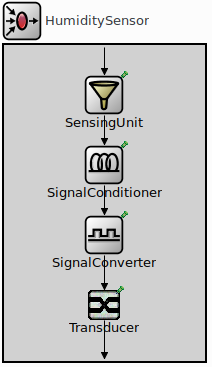
\includegraphics[width=0.3\textwidth]{sensor}
\end{figure}

\subsection{Wakeupreceiver}

Der Wakeupreceiver implementiert den Network interface controller\\ Nic802154\_TI\_CC2420A. Dieser nutzt den IEEE-Standard 802.15.4 mit einem CC2420 Receiver. Zusätzlich wurde der NIC um eine die Funktionen eines Wakeuprecievers erweitert. Dadurch kann Energie gespart werden, indem der Haupttransreceiver über einen bestimmten Zeitraum abgeschaltet wird. Mit dem Wakeupreceiver kann auch in diesem Zeitraum ein Wakeuppacket empfangen werden. Wenn dieses empfangen wurde wird der Haupttransreceiver wieder eingeschaltet werden und der normale Nachrichtenverkehr kann stattfinden.\\
Für die Implementierung wurden zusätzliche Parameter eingeführt. Zum einen beispielsweise setupWakeupCurrent und wakeupCurrent, mit denen der Energieverbrauch des Funkmoduls während der Ruhephasen definiert werden kann. Das Modul Wakeup\_Nic802154\_TI\_CC2420A enthält die komplette Definition des Wakeupreceivers. Die dazugehörigen Module und Klassen befinden sich im Omnet++-Modul \\ WakeUpRecv.

\begin{figure}[htbp]
\centering
\caption{Aufbau Wakeup-Nic}
\label{fig:routingbsp}
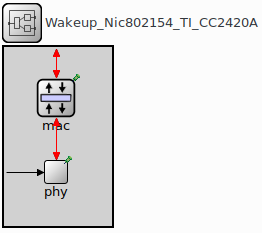
\includegraphics[width=0.3\textwidth]{wakeupnic}
\end{figure}

\section{Transportlayer}
\subsection{CustomWiseRoute - Baum}
Das Modul CustomWiseRoute ist eine Erweiterung des Mixim-Modul WiseRoute und daher ebenfalls ein Networklayer. Dieses erstellt eine Routingtabelle anhand einer gegebenen Adjazenzliste. Das Routing kann dabei zum Beispiel einen Baum beschreiben. Diese muss in Form eines Arrays definiert werden. In Abbildung \ref{fig:routingbsp} ist das Netzwerk als Zeichnung dargestellt.

\begin{minipage}{\textwidth}
\begin{lstlisting}
#node id     =  0  1  2  3  4  5  6  7  8  9 10 11
**.routeTree = "0  0  1  1  1  0  5  5  5  0  9  9"
\end{lstlisting}
\end{minipage}

Dabei wird für jeden Knoten der Vaterknoten definiert. Für jeden Knoten kann also nur 1 Vater definiert werden. Ein Knoten der die Wurzel eines Baumes darstellt wird die eigene Knotenadresse gesetzt.\\
Im Beispiel ist der Wurzelknoten der Knoten mit der Adresse 0. An diesem hängen die Knoten 1, 5 und 9. An diesen 3 Knoten hängen wiederum jeweils einige Knoten. Für die Adressauflösung muss für jeden Knoten eine Adresse wie folgt definiert werden:

\begin{minipage}{\textwidth}
\begin{lstlisting}
network.node.arp.offset = 0
\end{lstlisting}
\end{minipage}

Wenn Nachrichten innerhalb des Netzwerkes versendet werden, dann werden diese je nach Zieladresse von Knoten zu Knoten weitergeleitet, bis sie an ihrem Zielknoten angekommen sind. Im Falle eines Broadcasts werden die Nachrichten an jeden Knoten einmal gesendet und von jedem Empfänger verarbeitet.

\begin{figure}[htbp]
\centering
\caption{Routing}
\label{fig:routingbsp}

\includegraphics[width=\textwidth]{tree}
\end{figure}

\subsection{ClusterApplWiseRoute - Application Clustering}
Die ClusterApplWiseRoute ist ebenfalls ein Networklayer. Dieser erbt von der Klasse CustomWiseRoute und dieser daher sehr ähnlich. Lediglich das forwarding von Nachrichten wurde ein wenig angepasst. Es werden ClusterMaster beispielsweise Nachrichten von der Datensenke stets an die Blattknoten weiterleiten. Ebenso gilt das in die entgegengesetzte Richting, falls die Nachrichten an den ClusterMaster selbst adressiert sind.\\
Die Datensenke und die Blattknoten dagegen werden niemals Nachrichten weiterleiten.

\section{Applicationlayer}

\paragraph{Für Szenario 1} wird der Application-Layer NoApplicationClusteringAppl verwendet. Dieser erbt von der CustomMatrixApplication. Diese wurde jedoch noch um  Sensorfunktionen erweitert. In Szenario 1 nehmen die Knoten regelmäßige Messungen vor. Sobald der Event sendToMaster ausgelöst wird lesen die Knoten ihre bisher gesammelten Messwerte aus und leeren den Speicher. Die Messdaten werden dann anhand der Routingtabelle zum Masterknoten gesendet. Die Knoten gehen in regelmäßigen Intervallen in den Schlafmodus und wachen ebenfalls regelmäßig wieder auf. In den Wachphasen kann dann der Event sendToMaster ausgeführt werden. Es findet die Kommunikation zwischen den Knoten statt und nach einer gewissen Zeit gehen alle Knoten wieder in den Schlafmodus zurück.

\paragraph{Für Szenario 2} werden drei verschiedene Application-Layer definiert. Zum einen der MasterClusterAppl, welcher von der CustomDiceApplication erbt. Dieser Application-Layer wird im Master-Knoten des Netzwerkes implementiert. Es gibt also nur einen Knoten pro Netzwerk mit dem MasterClusterAppl.\\
Der ClusterMasterClusterAppl wird dem Master innerhalb des jeweiligen Clusters zugewiesen. Dieser erbt von CustomMatrixApplication. Er steuert das Verhalten des ApplicationClustering. Er kann die Knoten des Clusters wecken. Deren Energieladezustand anfordern und Messungen in den Knoten delegieren.\\
In allen Knoten die weder der Netzwerk-Master noch einer der Cluster-Master wird der LeafClusterAppl verwendet, welcher ebenfalls von CustomMatrixApplication erbt.   Dieser hört auf Pakete vom Cluster-Master und gibt seinen Energieladezustand und Messwerte an diesen, falls diese angefordert werden.

\paragraph{Für Szenario 3} wurde der Szenario3Appl definiert, welcher dem NoApplicationClusteringAppl aus Szenario 1 sehr ähnlich ist. Im Unterschied zu diesem wurde jedoch der Wechsel zwischen Wach- und Schlafmodus des Funktransreceivers geändert. Dies erfolgt hier nicht mehr zeitgesteuert, sondern wird durch Nachrichten ausgelöst.\\
Blattknoten können ihre Messungen durchführen. Sobald diese ihre Messungen senden wollen können sie ein WakeUpPacket an den nächsten Knoten schicken und anschließend ihre Nachricht senden.

\chapter{Testanwendungen}
Es sollten drei verschiedene Testanwendungen implementiert werden. Diese sollten zum Beispiel Energieverbrauch, Netzwerklebenszeit und ausgefallene Knoten unter verschiedenen Bedingungen erfassen.\\
\section{Szenario 1}
In der ersten Anwendung sollten die Sensorknoten in regelmäßigen Intervallen Messungen mit den jeweils vorhandenen Sensoren durchführen. Dabei sollte zu den entsprechenden Zeitpunkten jeder Knoten alle seine Messwerte erfassen und diese über einen einfachen Routingalgorithmus wie zum Beispiel eine Baumstruktur an die Datensenke übermitteln.
\paragraph{Umsetzung}
Das Netzwerk Szenario1 besteht aus 20 Knoten vom Type \\Sensor\_Wakeup\_DicePhyMacHost. Diese bilden eine Baumstruktur, wobei 4 Knoten am Wurzelknoten hängen. Die restlichen Knoten hängen wiederum an einem dieser 4 Knoten. Alle Knoten besitzen den Applicationlayer vom Typ NoApplicationClusteringAppl. Dieser ermöglicht das zeitgleiche aufwachen und einschlafen der Knoten und steuert das Versenden von Nachrichten in den Wachphasen. \\
Der Nachrichtenverkehr wird außerdem vom Networklayer CustomWiseRoute gesteuert. Dieser regelt das Routing nach der Baumstruktur, welche in Abbildung \ref{fig:nwds} zu sehen ist. Das Netzwerk kann mit dem Parameter routeTree definiert werden.

\begin{figure}[htbp]
\centering
\caption{Netzwerk der Szenarios}
\label{fig:nwds}
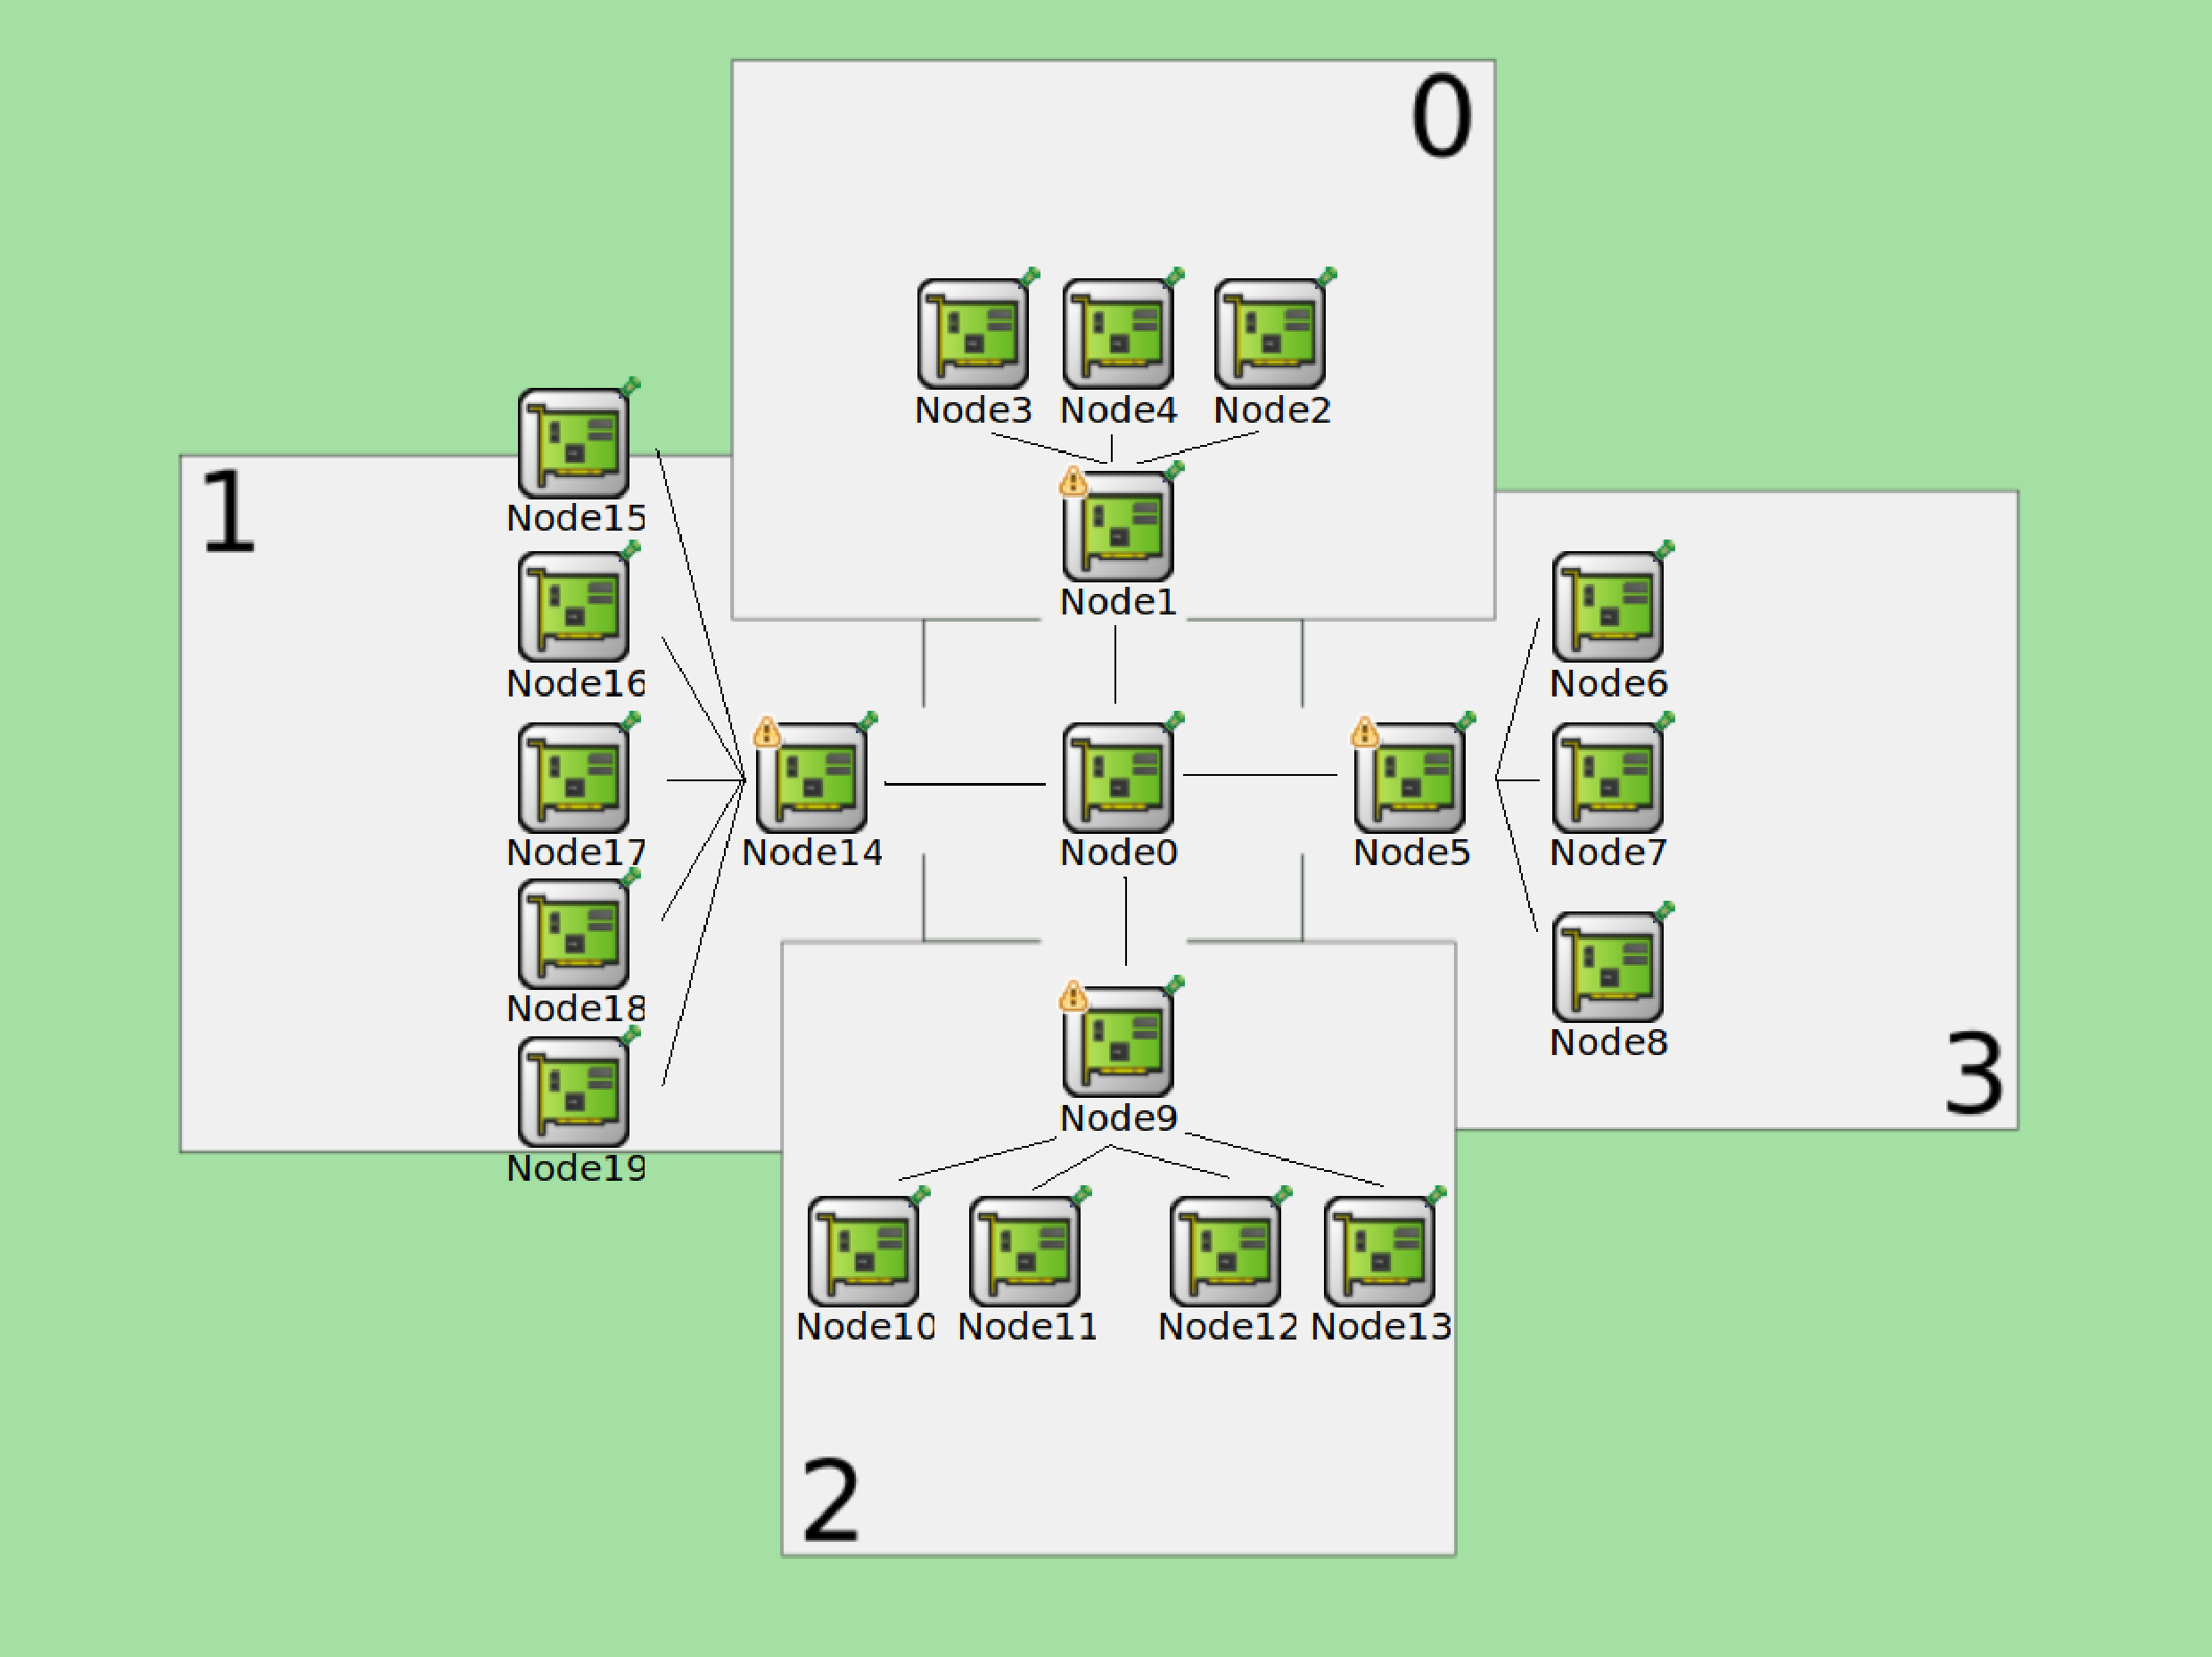
\includegraphics[width=\textwidth]{network}
\end{figure}

Die Knoten nehmen regelmäßige Messungen vor. Der Intervall für eine Messung kann im Parameter sensingIntervall definiert werden und ist auf den Wert von 10 Sekunden gesetzt. Alle 30 Sekunden wechseln alle Knoten in den Wachmodus und die Blattknoten senden ihre Messwerte, also jeweils 3 Stück pro Knoten, Sensor und Intervall. Bis die Messwerte übermittelt werden sind diese innerhalb des Memory-Moduls aus SensorTechnology gespeichert.

\section{Szenario 2}
In Anwendung Zwei sollten die Knoten in App-Cluster unterteilt werden. Die Funktionsweise ist in Abschnitt 2.2.2 beschrieben. Es misst also im Vergleich zum ersten Szenario nicht jeder Knoten, sondern es wird pro Cluster jeder Messwert nur einmal pro Zeitpunkt erhoben.
\paragraph{Umsetzung}
In Szenario 2 ist der Aufbau des Netzwerks analog zu dem in Szenario 1. Die Knoten sind ebenfalls wie in Abbildung \ref{fig:nwds} beschrieben angeordnet. Allerdings besitzen nicht alle Knoten den selben Applicationlayer. Es wird stattdessen in Datensenke, Masterknoten eines Clusters und normale Knoten eines Clusters unterschieden. Das genaue Verhalten dieser Applicationlayer ist im Abschnitt 2.3. (Applicationlayer) beschrieben.\\
Eine Messung wird in diesem Szenario durch die Datensenke gestartet. Dabei wird zunächst eine Wakeup-Message an alle Knoten gesendet. Anschließend fragen die Clustermaster-Knoten den Ladezustand der zugehörigen Knoten im Cluster ab. Die Sensoren die ein einzelner Knoten besitzt werden durch den Clustermaster einmalig zu Beginn der Simulation abgefragt. \\
Mit diesen beiden Informationen wählt der Clustermaster nun bis zu 4 Knoten aus, die abhängig von ihrer restlichen Energie und den Sensoren die jeweils höchste Restladung für einen Sensortyp besitzen. Diese Knoten werden danach vom Clustermaster mit dem Messen den entsprechenden Wertes beauftragt und erhalten im Anschluss daran den gemessenen Wert als Antwort.\\
Wenn alle 4 Messwerte des Clusters bestimmt wurden werden diese in einer gesammelten Nachricht zur Datensenke gesendet.

\section{Szenario 3}
In Anwendung Drei sollten die Knoten in wie in Szenario 1 strukturiert werden. Allerdings sollten nicht alle Knoten zu einem bestimmten Zeitpunkt aufwachen, sondern nur sobald ein Blattknoten seine Messungen übermitteln möchte. Dazu sollte der Blattknoten ein WakeUpPacket senden, um die Knoten auf dem Weg zur Datensenke zu wecken.
\paragraph{Umsetzung}
Auch Szenario 3 ist wie in Abbildung \ref{fig:nwds} aufgebaut. Auch sonst ist dem Szenario 1 sehr ähnlich. Der einzige Unterschied liegt im Applicationlayer. Wie in Abschnitt 2.3. (Applicationlayer) beschrieben werden vor jedem Nachrichtenverkehr Wakeup-Nachrichten versendet um die betroffenen Knoten zu wecken. Die Knoten des Netzwerks werden nicht alle zeitgesteuert geweckt. Dadurch ist es möglich das nur ein Teil der Knoten des Netzwerkes in den Wachmodus wechselt, falls zwischen diesen Knoten Nachrichten versendet werden sollen und die Knoten die nicht betroffen sind können weiter im Schlafmodus bleiben.